\documentclass[../report.tex]{subfiles}

\begin{document}

\begin{figure}[H]
\centering
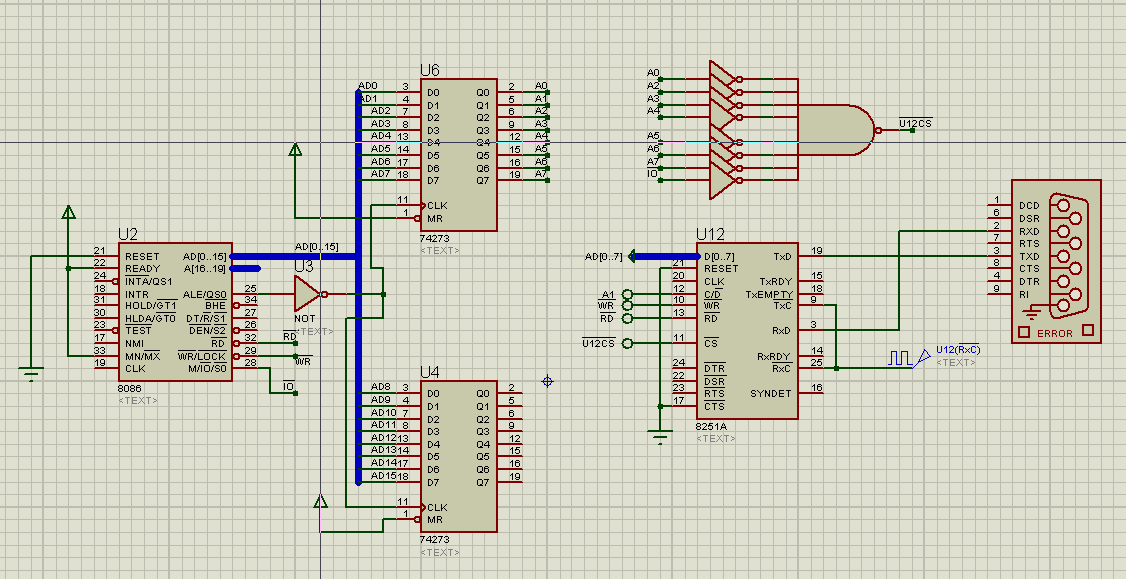
\includegraphics[width=\textwidth]{figures/diagram.png}
\caption{Sơ đồ mắc nối mạch (tổng thể).}
\end{figure}

\noindent Mạch bao gồm: 
\begin{itemize}
\item Một CPU 8086.
\item Hai bộ chốt địa chỉ 74273.
\item Một chip 8251.
\item Một cổng Compim.
\item Một mạch giải mã địa chỉ. 
\end{itemize}

\begin{figure}[H]
\centering
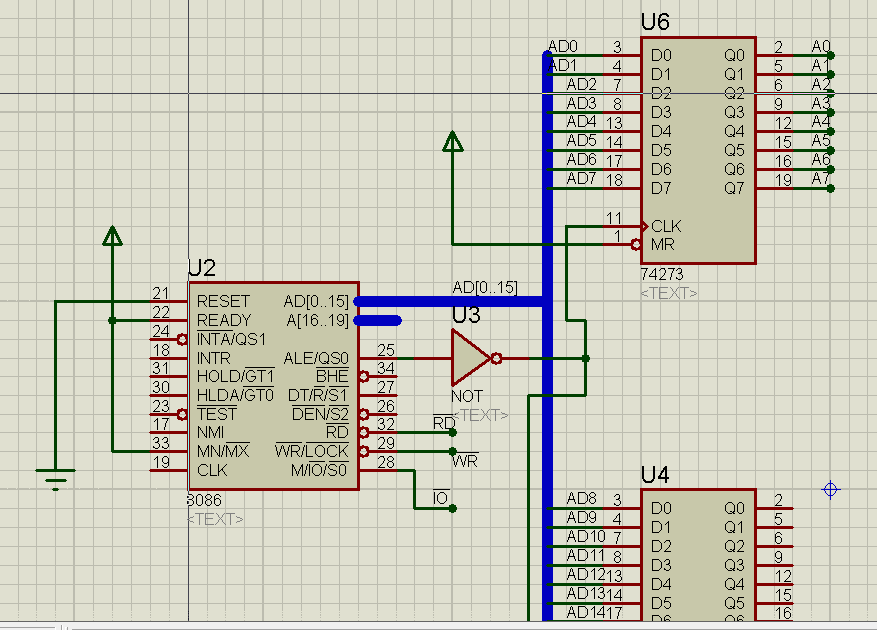
\includegraphics[width=\textwidth]{figures/diagram-left.png}
\caption{Sơ đồ mắc nối mạch (trái).}
\end{figure}

\begin{figure}[H]
\centering
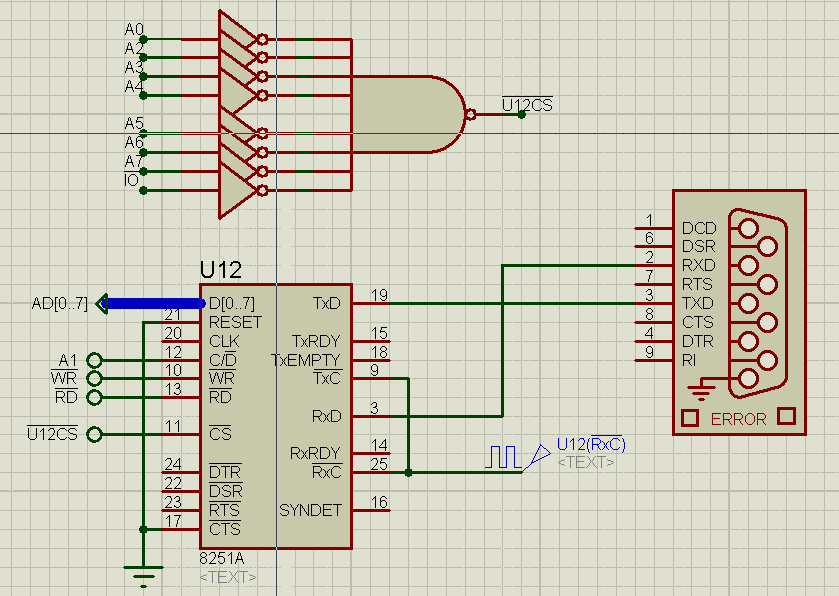
\includegraphics[width=\textwidth]{figures/diagram-right.png}
\caption{Sơ đồ mắc nối mạch (phải).}
\end{figure}

\begin{itemize}
\item[-] Mạch giải mã địa chỉ cho phép 2 địa chỉ là 0x00 và 0x02. \\
\item[-] Xung đồng hồ được sử dụng có tần số 19200Hz
\end{itemize}

\end{document}
